\documentclass{article}
\usepackage{amsmath}
\usepackage{url}
\usepackage{graphicx}
\usepackage{subcaption}
\title{Contextual BO experiment}
\author{Feng Zhao}

\begin{document}
\maketitle
\section{Experiment 1}
Using Contextual BO to find the maximal value of $f(x,a)$ for given $x$.
\begin{equation}\label{eq:f}
    f(x,a) = \cos(2 x) \cos(a) + \sin(x)
\end{equation}
Choosing $x,y \in [0,6]$.
In this experiment, $x$ is treated as task while $a$ is treated
as action.

Our goal is to provide a surrogate model of $z=g(x)=\arg\max_{a} f(x,a)$.
The exact solution is non-continuous, which means that it is very hard to estimate $z=g(x)$ at the
non-continuous points. Therefore, we need to sample more points in these places.
Bayesian optimization accomplishes this goal,
which can be verified by the histogram of samples $x$.

\begin{figure}[!ht]
    \begin{subfigure}[b]{0.49\textwidth}
        \centering
        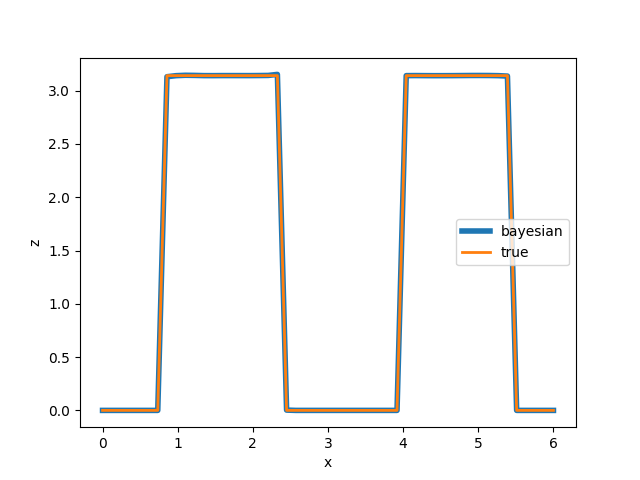
\includegraphics[width=\textwidth]{./cbo_1.png}
        \caption{Fitting result}
        \label{fig:rk_order_compare}
    \end{subfigure}~
    \begin{subfigure}[b]{0.49\textwidth}
      \centering
      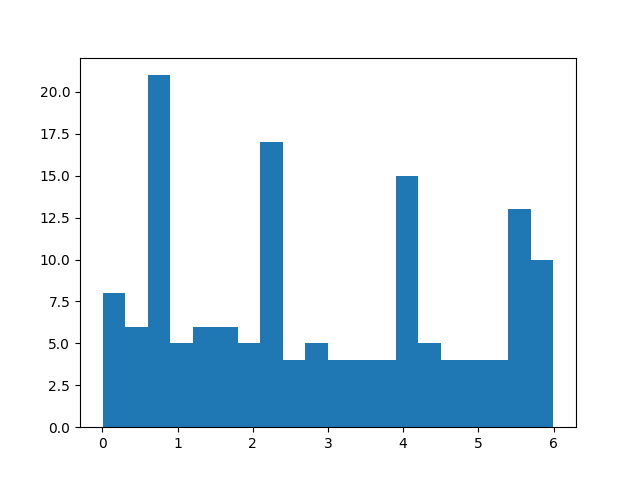
\includegraphics[width=\textwidth]{./cbo_1_hist.png}
      \caption{Histogram}
      \label{fig:time_equal_verify}
    \end{subfigure}
    \caption{}
\end{figure}

\section{Experiment 2}
Using the same object function but the adopted action should
satisfy the constraints.
\begin{equation}
    \cos(x)  \cos(a) - \sin(x) \sin(a) + 0.5 \leq 0    
\end{equation}
The optimal action is not unique in this constraint
setting, we plot $f(x,z)$ against $x$ instead.

\begin{figure}[!ht]
    \centering
    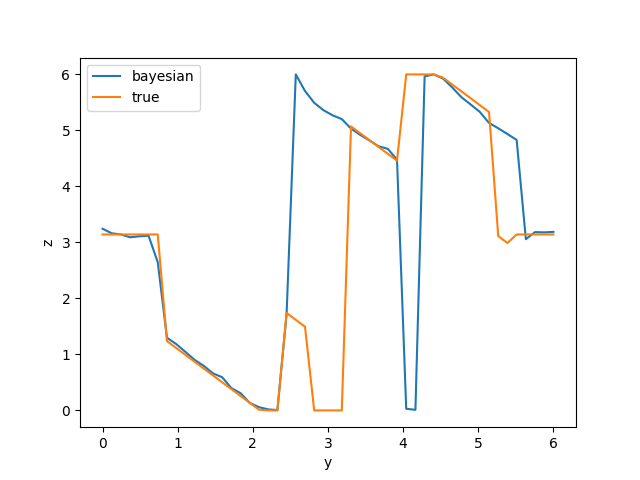
\includegraphics[width=6cm]{cbo_2.png}
\end{figure}
\end{document}


